%%%%%%%%%%%%%%%%%%%%%%%%%%%%%%%%%%%%%%%%%%%%%%%%%%%%%%%%%%%%%%%%%%%%
% Umsetzung
%%%%%%%%%%%%%%%%%%%%%%%%%%%%%%%%%%%%%%%%%%%%%%%%%%%%%%%%%%%%%%%%%%%%

\chapter{Umsetzung}
  \label{Umsetzung}
  
\section{Unity-Integration}
Als Ausgangspunkt liegt eine voll funktionsfähige Navigations-App für Bibliotheken vor. Sie wurde komplett in Unity umgesetzt. Die Einbindung der Orientierungsberechnung kann nicht direkt in Unity vorgenommen werden, da in Unity nur ein eingeschränkter Zugang auf die Cocoa-Frameworks, die die APIs zum Zugriff auf die Hardware zur Verfügungs stellen, möglich ist. Darum wird die App ohne den Hardwarezugriff als Xcode Projekt exportiert. Dann muss in Xcode ein Plug-in programmiert werden, das als Schnittstelle zwischen selbst geschriebenem Objective-C-Code in Xcode, der die Hardware ausließt, und Unity dient. Dazu muss erst noch in Unity das Plug-in als Eingabe-Skript erstellt werden. Dieses Eingabe-Skript ist in C\# geschrieben.
~\\
\begin{lstlisting}[float=htb, caption=Plug-in in Unity, label=listing001]
[DllImport ("__Internal")]
private static extern CMQuaternion getDeviceMotion();
\end{lstlisting}
  
In Listing \ref{listing001}  wird also die externe Methode \texttt{getDeviceMotion()} aufgerufen. Das Plug-in erwartet den Datentyp \texttt{CMQuaternion}. Später wird ein Quaternion übergeben, also immer die aktuelle absolute Orientierung. \texttt{CMQuaternion} ist eigentlich ein Datentyp auf dem Core Motion Framework und somit Unity nicht bekannt. Darum muss erst noch ein \texttt{struct} mit der Bezeichung \texttt{CMQuaternion} definiert werden (Listing \ref{listing002}).
~\\
\begin{lstlisting}[float=htb, caption=Struct \texttt{CMQuaternion} in C\#, label=listing002]
public struct CMQuaternion {
	public double x, y, z, w;
}
\end{lstlisting}

Alles weitere erfolgt jetzt direkt in Xcode. In Xcode wird eine \texttt{*.mm}-Datei angelegt zusammen mit der zugehörigen \texttt{*.h}-Datei. In der \texttt{*.mm}-Datei erfolgt die ganze Implementierung. Damit in der bestehenden App überhaupt Daten, die hier berechnet werden ankommen, muss als erstes die \texttt{getDeviceMotion()}-Methode implementiert werden:
~\\
\begin{lstlisting}[float=htb, caption=Methode \texttt{getDeviceMotion}, label=listing003]
static GyroscopeData* delegateObject = nil;

extern "C" {

	CMQuaternion getDeviceMotion () {

		if (delegateObject == nil) {
			delegateObject = [[GyroscopeData alloc] init];
		}
		
		return [delegateObject getOrientation];(*@\label{line001}@*)
	}    
}
\end{lstlisting}

Allerdings muss in dieser \texttt{extern  C }-Umgebung in C geschrieben werden. In C sind aber die API-Aufrufe nicht oder nur sehr umständlich möglich. Darum wird in Zeile \ref{line001} in Listing \ref{listing003} eine weitere Methode \texttt{getOrientation} aufgerufen. 
~\\
\begin{lstlisting}[float=htb, caption=Methode \texttt{getOrientation}, label=listing004]
- (CMQuaternion)getOrientation {
	...
	...
}
\end{lstlisting}

Diese Methode (Listing \ref{listing004})  enthält den eigentlichen Objective-C-Quellcode. In ihr können alle API-Aufrufe problemlos ausgeführt werden. 

In Abbildung \ref{fig:unity-integration} wird der Zusammengang der Methoden und Dateien nochmal schematisch dargestellt.

\cite{unity}

\begin{figure}[htb]
\centering
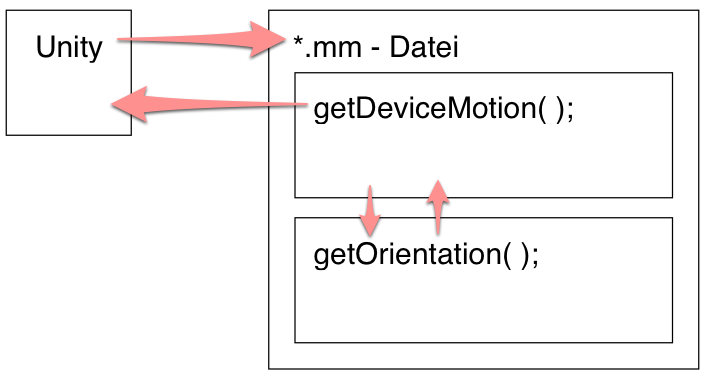
\includegraphics[scale=0.5]{figures/unity-integration}
\caption{Unity-Integration}
\label{fig:unity-integration}
\end{figure}
  
\section{Vorbereitung der nötigen Daten}
Um die Multidatenfusion durchführen zu können, müssen erst alle nötigen Daten ausgelesen werden. Dazu müssen \texttt{CMMotionManager}- und \texttt{CLLocationManager}-Objekte initialisert werden.  \cite{book001} \cite{book002} 
~\\
\begin{lstlisting}[float=htb, caption=\texttt{locationManager} und \texttt{motionManager} initialisieren \cite{apple:003}, label=listing005]
// Set up locationManager
if (locationManager == nil) {
	locationManager=[[CLLocationManager alloc] init];
	locationManager.desiredAccuracy = kCLLocationAccuracyBest;(*@\label{line002}@*)
}
    
// Set up motionManager    
if (motionManager == nil) {
	motionManager = [[CMMotionManager alloc] init];
	motionManager.deviceMotionUpdateInterval = 1.0/60.0;(*@\label{line003}@*)
}
\end{lstlisting}

In Zeile \ref{line002} in Listing \ref{listing005} wird die Genauigkeit des \texttt{CLLocationManager}-Objekts und in Zeile \ref{line003} die Update-Frequenz des \texttt{CMMotionManager}-Objekts eingestellt. Der Kompass-Wert, der aus dem \texttt{CLLocationManager}-Objekt ausgelesen wurde, muss sehr genau sein.

Das Auslesen des Kompass-Werts findet eventgesteuert statt. Ein neuer Wert wird nur dann ausgelesen, wenn er sich vom alten Wert unterscheidet. Dazu wird die minimale Winkeländerung auf $1^o$ festgesetzt.
~\\
\begin{lstlisting}[float=htb, caption=\texttt{locationManager} starten \cite{apple:003}, label=listing006]
// Start listening to events from locationManager
if ([CLLocationManager headingAvailable]) {
	locationManager.headingFilter = 1;
	[locationManager startUpdatingHeading];(*@\label{line004}@*)
}
\end{lstlisting}

Mit dem Aufrufen der Methode \texttt{startUpdatingHeading} in Zeile \ref{line004} in Listing \ref{listing006} wird hier auch gleichzeitig das eventgesteuerte Abfragen des Kompass-Werts gestartet.

Die Methode, die auf die Kompass-Änderungen (Listing \ref{listing007}) hört, liest den Kompass-Wert aus und stellt ihn in einer globalen Variable zur Verfügung.
~\\
\begin{lstlisting}[float=htb, caption=Azimut ermittelt durch Kompass, label=listing007]
- (void)locationManager:(CLLocationManager *)manager didUpdateHeading:(CLHeading *)newHeading {
	// Get new heading
	mHeading = newHeading.magneticHeading;    
    
	//location specific offset depending on the 3D model
	locationOffset = 90;
	mHeading += locationOffset;
    
	if (mHeading > 360) {
		mHeading -= 360;
	}
	else if (mHeading < 0) {
		mHeading += 360;
	}
}
\end{lstlisting}

Es kann vorkommen, dass in dem 3D-Modell des Raums nicht an der selben Stelle Norden ist wie in der Realität an diesem Ort. Darum muss, wenn dieser Fall auftritt, ein Offset zu dem ausgelesenen Wert addiert werden. Das Resultat kann ein Wert sein, der entweder größer als $360^o$ oder kleiner als $0^o$ ist. Der Wert muss dann normalisiert werden indem $360^o$ subtrahiert oder addiert werden. Das Ergebnis ist der Azimut-Wert, ermittelt durch den Kompass.

Die Azimut-Änderung, ermittelt durch das Gyroskop und die Elevation, liefert das \texttt{CMMotionManager}-Objekt.
~\\
\begin{lstlisting}[float=htb, caption=Bewegungsdaten auslesen \cite{apple:003}, label=listing008]
if(motionManager.isDeviceMotionAvailable) {
        
	// Listen to events from the motionManager
	motionHandler = ^ (CMDeviceMotion *motion, NSError *error) {
	
	CMAttitude *currentAttitude = motion.attitude;(*@\label{line005}@*)
	.
	.
	.
}
\end{lstlisting}

Im \texttt{CMDeviceMotion}-Objekt werden Messungen des Accelerometers und des Gyroskops zusammengefasst. Der \texttt{motionHandler} wird immer dann aufgerufen, wenn es Bewegungs-Daten des Geräts zu verarbeiten gibt. Hier ist das alle 1/60 Sekunden der Fall, weil das bei der Initialisierung des \texttt{CMMotionManager}-Objekts so festgelegt wurde.

Das Auslesen der eigentlichen Orientierungsdaten erfolgt in Zeile \ref{line005} von Listing \ref{listing008}. Wobei in diesem \texttt{CMAttitude}-Objekt alle drei Beschreibungs-Möglichkeiten, Euler-Winkel, Rotationsmatrix und Quaternion, zusammengefasst sind.
~\\
\begin{lstlisting}[float=htb, caption=Azimut-Änderung berechnen, label=listing009]
quaternion = currentAttitude.quaternion;

if (oldQuaternion.w != 0 || oldQuaternion.x != 0 || oldQuaternion.y != 0 || oldQuaternion.z != 0){
	diffQuaternion = [self multiplyQuaternions:[self inverseQuaternion:oldQuaternion] :quaternion];
	diffQuaternion = [self normalizeQuaternion:diffQuaternion];
}            
oldQuaternion = quaternion;
\end{lstlisting}

Die Orientierung wird als Queternion ausgelesen und die Differenz zur letzten Orientierung gespeichert. Dies wird erreicht indem der inverse Quaternion des alten Werts mit dem Quaternion des neuen Werts multipliziert wird. Danach muss das Ergebnis noch normalisiert werden. Das geschieht in Listing \ref{listing009} mit Hilfe der vier Methoden \texttt{quaternionMagnitude} (Listing \ref{listing010}), \texttt{inverseQuaternion} (Listing \ref{listing011}), \texttt{multiplyQuaternions} (Listing \ref{listing012}) und \texttt{normalizeQuaternion} (Listing \ref{listing013}).
~\\
\begin{lstlisting}[float=htb, caption=Methode \texttt{quaternionMagnitude}, label=listing010]
- (float) quaternionMagnitude:(CMQuaternion)inputQuaternion {
	float magnitude = sqrt(inputQuaternion.w*inputQuaternion.w + inputQuaternion.x*inputQuaternion.x + inputQuaternion.y*inputQuaternion.y + inputQuaternion.z*inputQuaternion.z);
	
	return magnitude;
}
\end{lstlisting}


\begin{lstlisting}[float=htb, caption=Methode \texttt{inverseQuaternion}, label=listing011]
- (CMQuaternion) inverseQuaternion:(CMQuaternion)inputQuaternion {
	float magnitude = [self quaternionMagnitude:inputQuaternion];
	
	quaternion.w = inputQuaternion.w/magnitude;
	quaternion.x = -inputQuaternion.x/magnitude;
	quaternion.y = -inputQuaternion.y/magnitude;
	quaternion.z = -inputQuaternion.z/magnitude;
	
	return quaternion;
}
\end{lstlisting}

\begin{lstlisting}[float=htb, caption=Methode \texttt{multiplyQuaternions}, label=listing012]
- (CMQuaternion) multiplyQuaternions:(CMQuaternion)quaternionA:(CMQuaternion)quaternionB {
	quaternion.w = quaternionA.w*quaternionB.w - quaternionA.x*quaternionB.x - quaternionA.y*quaternionB.y - quaternionA.z*quaternionB.z;
	quaternion.x = quaternionA.w*quaternionB.x + quaternionA.x*quaternionB.w - quaternionA.y*quaternionB.z + quaternionA.z*quaternionB.y;
	quaternion.y = quaternionA.w*quaternionB.y + quaternionA.x*quaternionB.z + quaternionA.y*quaternionB.w - quaternionA.z*quaternionB.x;
	quaternion.z = quaternionA.w*quaternionB.z - quaternionA.x*quaternionB.y + quaternionA.y*quaternionB.x + quaternionA.z*quaternionB.w;

	return quaternion;
}
\end{lstlisting}

\begin{lstlisting}[float=htb, caption=Methode \texttt{normalizeQuaternion}, label=listing013]
- (CMQuaternion) normalizeQuaternion:(CMQuaternion)inputQuaternion {
	float magnitude = [self quaternionMagnitude:inputQuaternion];
	
	quaternion.w = inputQuaternion.w / magnitude;
	quaternion.x = inputQuaternion.x / magnitude;
	quaternion.y = inputQuaternion.y / magnitude;
	quaternion.z = inputQuaternion.z / magnitude;
	
	return quaternion;
}
\end{lstlisting}

Die interessanten Werte, Azimut und Elevation, werden aus dem Quaternion in Grad berechnet. Die Methoden \texttt{azimutFromQuaternion} (Listing \ref{listing014}) und \texttt{elevationFromQuaternion}  (Listing \ref{listing015}) berechnen den entsprechenden Winkel in Radian.
~\\
\begin{lstlisting}[float=htb, caption=Azimut-Wert aus Quaternion berechnen, label=listing014]
- (float) azimutFromQuaternion:(CMQuaternion)quaternion {
	float azimut = atan2(2*(quaternion.w*quaternion.z+quaternion.x*quaternion.y), 1 - 2*(quaternion.y*quaternion.y+quaternion.z*quaternion.z));
	return azimut;
}

azimutDiff = RADIANS_TO_DEGREES([self azimutFromQuaternion:diffQuaternion]);
\end{lstlisting}

\begin{lstlisting}[float=htb, float=htb, caption=Elevation-Wert aus Quaternion berechnen, label=listing015]
- (float) elevationFromQuaternion:(CMQuaternion)quaternion {
	float elevation = atan2(2*(quaternion.w * quaternion.x + quaternion.y * quaternion.z), 1-2 * (quaternion.x * quaternion.x + quaternion.y * quaternion.y));
	return elevation;
} 

elevation = -[self elevationFromQuaternion:quaternion];
elevation += M_PI/2;
elevation = RADIANS_TO_DEGREES(elevation);
\end{lstlisting}

Bei der Elevation muss noch eine Korrektur von $90^o$ vorgenommen werden. Denn wenn man das iPad mit dem Display nach oben um $90^o$ neigt, sodass das Display zum Betrachter zeigt, befindet sich standardmäßig genau in dieser Position der Sprung von $0^o$ auf $360^o$. Um eventuellen Problemen mit dieser Tatsache aus dem Weg zu gehen, wird der Sprung um $90^o$ nach oben verschoben. Dann tritt er nur auf wenn der Betrachter das iPad direkt an die Decke hält. \cite{paper:001} \cite{mathworks}

\section{Multisensordatenfusion}
Nur der Azimut-Wert muss noch selbst berechnet werden. Das Core Motion-Framework liefert bereits einen mit dem Accelerometer stabilisierten Elevation-Wert. Darum weist der in Listing \ref{listing015} berechnete Elevation-Wert keinen bemerkbaren Drift mehr auf.

Nun kann die Formel aus Kapitel \ref{formula001} umgesetzt werden.
~\\
\begin{lstlisting}[float=htb, caption=Eigentliche Datenfusion, label=listing016]
updatedAzimut = updatedAzimut - azimutDiff;(*@\label{line006}@*)

float alpha = 19.0;
float phi = 1.0;

//fusionate gyro estimated heading with new magneticHeading
updatedAzimut = (alpha* updatedAzimut + phi*heading)/(alpha+phi);(*@\label{line007}@*)         
\end{lstlisting}

In Zeile \ref{line006} aus Listing \ref{listing016} wird die Azimut-Änderung auf den vorherigen Azimut-Wert angewendet. Zeile \ref{line007} ist die genaue Umsetzung der Formel aus Kapitel \ref{formula001}. \texttt{updatedAzimut} ist der zur Drehung verwendete Azimut-Wert korrigiert um die Drehung seit dem letzten Wert. \texttt{heading} ist der durch den Kompass bestimmte Azimut-Wert. Mit den beiden Steuerungsvariablen \texttt{alpha} und \texttt{phi} wird gesteuert welche Anteile die jeweiligen Komponenten der Fusion haben.
~\\
\begin{lstlisting}[float=htb, caption=Generierung des Endergebnisses, label=listing017]
rotation = [self createFromAxisAngle:0 :elevation :DEGREES_TO_RADIANS(updatedAzimut)];
return rotation;
\end{lstlisting}
~\\
\begin{lstlisting}[float=htb, caption=Generierung eines Quaternions aus Euler-Winkeln, label=listing018]
- (CMQuaternion) createFromAxisAngle:(double)roll:(double)pitch:(double)yaw {
	CMQuaternion quaternion;
	
	float num9 = roll * 0.5f;
	float num6 = (float) sin((double) num9);
	float num5 = (float) cos((double) num9);
	float num8 = pitch * 0.5f;
	float num4 = (float) sin((double) num8);
	float num3 = (float) cos((double) num8);
	float num7 = yaw * 0.5f;
	float num2 = (float) sin((double) num7);
	float num = (float) cos((double) num7);
	quaternion.w = ((num * num3) * num5) + ((num2 * num4) * num6);
	quaternion.x = ((num * num4) * num5) + ((num2 * num3) * num6);
	quaternion.y = ((num2 * num3) * num5) - ((num * num4) * num6);
	quaternion.z = ((num * num3) * num6) - ((num2 * num4) * num5);
	
	return quaternion;
}
\end{lstlisting}

Mit Listing \ref{listing017} wird das Ergebnis zusammengefasst. Aus \texttt{elevation} und \texttt{updatedAzimut} wird mittels der Methode \texttt{createFromAxisAngle} (Listing \ref{listing018}) der Quaternion \texttt{rotation} generiert. Er ist die Rückgabe dieser Funktion und wird vom Plug-in in Unity erwartet.

\section{Test-App}
\begin{figure}[htb]
\centering
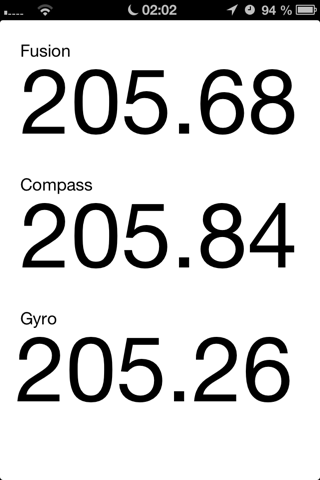
\includegraphics[scale=0.6]{figures/testapp}
\caption{Test-App}
\label{fig:testapp001}
\end{figure}
Um die folgenden Messungen und Grafiken für den Ergebnis-Teil zu ermitteln, wurde eine eigene Test-App erstellt. Diese teilt sich mit der Navigations-App den selben Quellcode bezüglich der Orientierung. Allerdings besteht die Test-App nur aus dem Code, der für die Orientierungsberechnungen wichtig ist, erweitert um eine Funktion, die die berechneten Werte in eine SQLite-Datenbank schreibt. Zusätzlich zeigt die App die drei relevanten Werte auch auf dem Display zur Kontrolle an. Immer wenn die App gestartet bzw. aufgerufen wird, wird eine neue Messung gestartet. Falls eine SQLite-Datei von einer vorherigen Messung noch vorhanden ist, wir diese überschrieben. Das Beenden der App durch Drücken des Home-Buttons beendet auch die Aufzeichnung der Werte. Die SQLite-Datei kann nun bequem aus iTunes heraus auf einem Computer zur Weiterverabreitung gespeichert werden.

